\documentclass[a4paper]{book}

%%% INICIO DEL PREÁMBULO %%%

\usepackage[utf8]{inputenc}
\usepackage[greek,spanish,es-tabla,es-nodecimaldot,es-noindentfirst]{babel}
\usepackage{babelbib}
\usepackage{nccmath}
\usepackage{amsthm}
\usepackage{lipsum}
\usepackage{tcolorbox}
\usepackage[thicklines]{cancel}
\usepackage{mathtools}
\usepackage{amssymb}
\usepackage{amsmath}
\usepackage{caption}
\usepackage{subcaption}
\usepackage{color}
\usepackage{verbatim}
\usepackage{enumerate}
\usepackage{geometry}
\geometry{a4paper,left=35mm,right=35mm,top=15mm,bottom=15mm}
\usepackage{isotope}
\usepackage{maybemath}
\usepackage{upgreek}
\usepackage{wasysym}
\usepackage[italic]{hepparticles}
\usepackage{subdepth}
\usepackage{siunitx}
\sisetup{
	mode 			= text,
	parse-units 	= false
}
\usepackage{physics}
\usepackage{braket}
\usepackage{tensor}
\usepackage{chemformula}
\usepackage{tikz}
\usepackage{url}
\usepackage{listings}
\usepackage{multirow}
\usepackage{multicol}
\usepackage[colorlinks=true]{hyperref}
\hypersetup{
	citecolor = blue,
	linkcolor = blue,
	urlcolor = blue,
	pdfauthor = {Javier Rodrigo López}
}
\usepackage{eso-pic}

% tikz
\usepackage{tikz} \usetikzlibrary{fit,babel,shapes,arrows,patterns,positioning,calc,decorations.pathmorphing,decorations.markings}
\tikzstyle{block} = [draw, fill=white, rectangle,
minimum height=3em, minimum width=6em]
\tikzstyle{sum} = [draw, fill=white, circle, node distance=1cm]
\tikzstyle{input} = [coordinate]
\tikzstyle{output} = [coordinate]
\tikzstyle{pinstyle} = [pin edge={to-,thin,black}]
\tikzset{
	block/.style = {draw, fill=white, rectangle, minimum height=3em, minimum width=3em},
	tmp/.style  = {coordinate},
	sum/.style= {draw, fill=white, circle, node distance=1cm},
	input/.style = {coordinate},
	output/.style= {coordinate},
	pinstyle/.style = {pin edge={to-,thin,black}}
}

\usepackage[oldvoltagedirection]{circuitikz}
\usepackage{pdflscape}

% Títulos
\usepackage{titlesec}
\titleformat{\section}{\normalfont\Large\bfseries}{\thesection}{1em}{}[{\titlerule[0.8pt]}]
% \renewcommand{\thesubsection}{\arabic{chapter}.\arabic{section}.\Alph{subsection}}
\titleformat{\subsubsection}{\normalfont\normalsize\bfseries}{\thesubsubsection}{1em}{}[{\titlerule[0.05pt]}]
\titlespacing{\section}{0pt}{2\parskip}{\parskip}
\titlespacing{\subsection}{0pt}{\parskip}{0pt}
\titlespacing{\subsubsection}{0pt}{\parskip}{0pt}

% Numeración de secciones
\setcounter{tocdepth}{2}
\setcounter{secnumdepth}{2}

% Figuras y descripciones
\renewcommand{\thefigure}{\arabic{figure}}
\renewcommand{\thesubfigure}{\Alph{subfigure}}
\captionsetup[figure]{labelfont={bf},name={Figura},labelsep=period}
\numberwithin{figure}{chapter}
\numberwithin{equation}{chapter}

% Enumerations
\newcounter{myenumi}
\renewcommand{\themyenumi}{\alph{myenumi})}
\newenvironment{myenumerate}{\setlength{\parindent}{0pt}\setcounter{myenumi}{0}\renewcommand{\item}{\par\refstepcounter{myenumi}\makebox[1.3em][l]{\themyenumi}}}{\par\bigskip\noindent\ignorespacesafterend}

% Own environments
\newenvironment{nota}{\underline{\textbf{NOTA:}} }{}
\newenvironment{caja}{\begin{tcolorbox}[colback = white, sharp corners, boxrule = 1 pt]}{\end{tcolorbox}}
\newtheorem*{conclusion}{Conclusión}
\newtheorem{teorema}{Teorema}
\newtheorem{definicion}{Definición}

% Para una bonita portada
\usepackage{wallpaper}
\usepackage{titling}
\usepackage{fancyhdr}
\pagestyle{fancy}
\setlength{\droptitle}{-10cm}
\renewcommand{\chaptermark}[1]{%
	\markboth{#1}{}}
\renewcommand{\sectionmark}[1]{%
	\markright{}}
\fancyhf{}
\fancyhead[LE,RO]{\bfseries\thepage} \fancyhead[LO]{\bfseries\rightmark} \fancyhead[RE]{\bfseries\leftmark} \renewcommand{\headrulewidth}{0pt} \renewcommand{\footrulewidth}{0pt} \addtolength{\headheight}{15pt}
\fancypagestyle{plain}{%
	\fancyhead{}
	\renewcommand{\headrulewidth}{0pt}
}

% Organización del texto
\newcommand{\formula}[1]{\vspace{13 pt}\noindent \textbf{\underline{#1}}}
\newcommand{\subtext}[1]{_{\text{#1}}}

% Unidades y utilidades varias
\renewcommand{\S}{\operatorname{S}}
\newcommand{\dB}{\operatorname{dB}}
\newcommand{\dBW}{\operatorname{dBW}}
\newcommand{\dBm}{\operatorname{dBm}}
\newcommand{\Hz}{\operatorname{Hz}}
\newcommand{\s}{\operatorname{s}}
\newcommand{\A}{\operatorname{A}}
\newcommand{\V}{\operatorname{V}}
\newcommand{\ohm}{\,\Omega}
\newcommand{\Pa}{\operatorname{Pa}}
\newcommand{\W}{\operatorname{W}}
\newcommand{\I}{\operatorname{I}}
\newcommand{\C}{\operatorname{C}}
\newcommand{\K}{\operatorname{K}}
\newcommand{\m}{\operatorname{m}}
\newcommand{\mm}{\operatorname{mm}}
\newcommand{\rad}{\operatorname{rad}}
\newcommand{\mol}{\operatorname{mol}}
\newcommand{\J}{\operatorname{J}}
\newcommand{\kg}{\operatorname{kg}}
\newcommand{\incremento}{\Delta}
\newcommand{\psus}{\, \ldots \,}
\newcommand{\mcm}{\operatorname{mcm}}
\newcommand{\MCD}{\operatorname{MCD}}
\renewcommand{\sin}{\sen}
\renewcommand{\arcsin}{\arcsen}
\renewcommand{\arctan}{\arctg}
\renewcommand{\min}{\operatorname{mín}}

\DeclarePairedDelimiter\evaluat{.}{\rvert}

% Vectores
\usepackage[c]{esvect}
\renewcommand{\vec}[1]{\vv{{#1}}}
\newcommand{\proy}[2]{\operatorname{proy}_{\vec{#2}}\vec{#1}}
\newcommand{\antiparallel}{\downharpoonleft \! \upharpoonright}
\newcommand{\parallelvec}{\upharpoonleft \! \upharpoonright}

% Espaciado
\usepackage{enumitem}
\setlist{before={\parskip=3pt}, after=\vspace{\baselineskip}}
\setlength{\parindent}{0pt}
\setlength{\parskip}{0.5em}

% Estadística
\DeclareMathOperator{\Var}{Var}
\DeclareMathOperator{\Cov}{Cov}
\renewcommand{\var}{\sigma ^2}
\DeclareMathOperator{\B}{B}
\DeclareMathOperator{\BN}{BN}
\DeclareMathOperator{\Geo}{Geo}
\DeclareMathOperator{\Poisson}{Poisson}
\DeclareMathOperator{\U}{U}
\DeclareMathOperator{\Exp}{Exp}
\DeclareMathOperator{\N}{N}
\DeclareMathOperator{\Mult}{Mult}
\newcommand{\TF}[1]{\mathrm{TF} \left\lbrace \left. #1 \right\rbrace \right.}
\newcommand{\probCond}[2]{P \left( #1 \: \middle\vert\:  #2 \right) }

% Electromagnetismo y Ondas
\newcommand{\errorGrave}{\textbf{FG!!!}}
\newcommand{\mas}{M.A.S.}
\newcommand{\mcu}{M.C.U.}
\newcommand{\ed}{E.D.}
\newcommand{\edmas}{E.D. del M.A.S.}
\usepackage{esint}

% Señales y Sistemas
\renewcommand{\H}{H}

% Circled number
\newcommand{\circledNumber}[1]{\raisebox{.9pt}{\textcircled{\raisebox{-.9pt}{#1}}}}

% Footnotes
% \renewcommand{\thefootnote}{\fnsymbol{footnote}}

% Ejemplo
\newcounter{elejemplo}
\newcommand{\ejemplo}[2]{
	\refstepcounter{elejemplo}
	\begin{center}
		\fbox{\begin{minipage}{0.85\linewidth}
			\textbf{Ejemplo \arabic{elejemplo}.} #1
			\begin{center}
				\underline{\textbf{Solución}}
			\end{center}
			#2
		\end{minipage}}
	\end{center}
}

% Repeticiones
\usepackage{forloop}
\newcommand{\repvec}[3]{
	\foreach \uwu in {1,...,#2}
		{\vec{#1}_{\uwu} ,}
	\, \ldots \, , \vec{#1}_{#3}
}
\newcommand{\rep}[3]{
	\foreach \uwu in {1,...,#2}
		{#1_{\uwu} ,}
	\, \ldots \, , #1_{#3}
}
\newcommand{\repinf}[3]{
	\foreach \uwu in {#2,...,#3}
		{#1_{\uwu} ,}
	\, \ldots
}

%%% FIN DEL PREÁMBULO %%% % Se incluye el preámbulo
\usepackage{etoolbox}
\makeatletter
\pgfcircdeclarebipole{}
    {\ctikzvalof{bipoles/tline/height}}{tline}
    {\ctikzvalof{bipoles/tline/height}}
    {\ctikzvalof{bipoles/tline/width}}
{   
    %% First find distance from startpoint to endpoint
    \pgfpointdiff{\pgfpointanchor{\ctikzvalof{bipole/name}start}{center}}
                 {\pgfpointanchor{\ctikzvalof{bipole/name}end}{center}}
    \pgfmathparse{veclen(\the\pgf@x,\the\pgf@y)}
    %% The coordinate system has been changed so that the origin is at the midpoint and
    %% the line is along the x axis. So shift back by half the length of the line, and 
    %% make the cylinder of width roughly the length of the line, with a 40pt setback
    %% on each side.
    \pgftransformxshift{\pgfmathresult/2-30pt}
    \pgf@circ@res@left=\dimexpr-\pgfmathresult pt+40pt\relax

    %% Here is the original function, copied directly from the source of circuittikz, 
    %% down to next %%
    \pgf@circ@res@step=.2\pgf@circ@res@right % half x axis
    \pgfsetlinewidth{\pgfkeysvalueof{/tikz/circuitikz/bipoles/thickness}\pgfstartlinewidth}
    \pgfpathmoveto{\pgfpoint{\pgf@circ@res@right-\pgf@circ@res@step}{\pgf@circ@res@up}}
    \pgfpathlineto{\pgfpoint{\pgf@circ@res@left+\pgf@circ@res@step}{\pgf@circ@res@up}}
    \pgfpatharc{-90}{90}{-\pgf@circ@res@step and -\pgf@circ@res@up}
    \pgfpathlineto{\pgfpoint{\pgf@circ@res@right-\pgf@circ@res@step}{\pgf@circ@res@down}}
    \pgfsetfillcolor{white}
    \pgfusepath{draw,fill}

    %% I have to fill the figure to block out the original line
    \pgfpathellipse{\pgfpoint{\pgf@circ@res@right-\pgf@circ@res@step}{0}}
                   {\pgfpoint{\pgf@circ@res@step}{0}}
                   {\pgfpoint{0}{-\pgf@circ@res@up}}
    \pgfsetfillcolor{white}
    \pgfusepath{draw, fill}

    %% Redraw part of the line that gets blocked by the cylinder by mistake
    \pgfsetlinewidth{\pgfstartlinewidth}
    \pgfpathmoveto{\pgfpoint{\pgf@circ@res@right-1*\pgf@circ@res@step}{0pt}}
    \pgfpathlineto{\pgfpoint{\pgf@circ@res@right}{0pt}}
    \pgfusepath{draw}
} % Para poder dibujar líneas de transmisión con circutikz

% Título y portada
\title{\Huge Teoría de la Comunicación\\\vspace*{5pt}
\Large Apuntes de clase}
\author{Javier Rodrigo López \thanks{Correo electrónico: \href{mailto:javiolonchelo@gmail.com}{\texttt{javiolonchelo@gmail.com}}}} 
\date{\today}

%%% INICIO DEL DOCUMENTO %%%
\begin{document}

\setlength{\wpYoffset}{-2 cm}
\ThisCenterWallPaper{0.5}{./Imágenes/La_magie_noir-Rene_Magritte.jpg}
\maketitle

% Marca de agua
\AddToShipoutPictureFG{
\begin{tikzpicture}[overlay,remember picture]
\path (current page.south west) -- (current page.north east)
 node[midway,scale=8,color=lightgray,sloped,opacity=0.05] {Javier Rodrigo López};
\end{tikzpicture}
}

% Logotipos UPM y ETSIST
\begin{figure}[t!]
\centering
	\begin{subfigure}[b]{0.65\linewidth}
		
\includegraphics[width=\linewidth]{../../Archivos comunes/upm_logo.png}
	\end{subfigure}
	\begin{subfigure}[b]{0.25\linewidth}
		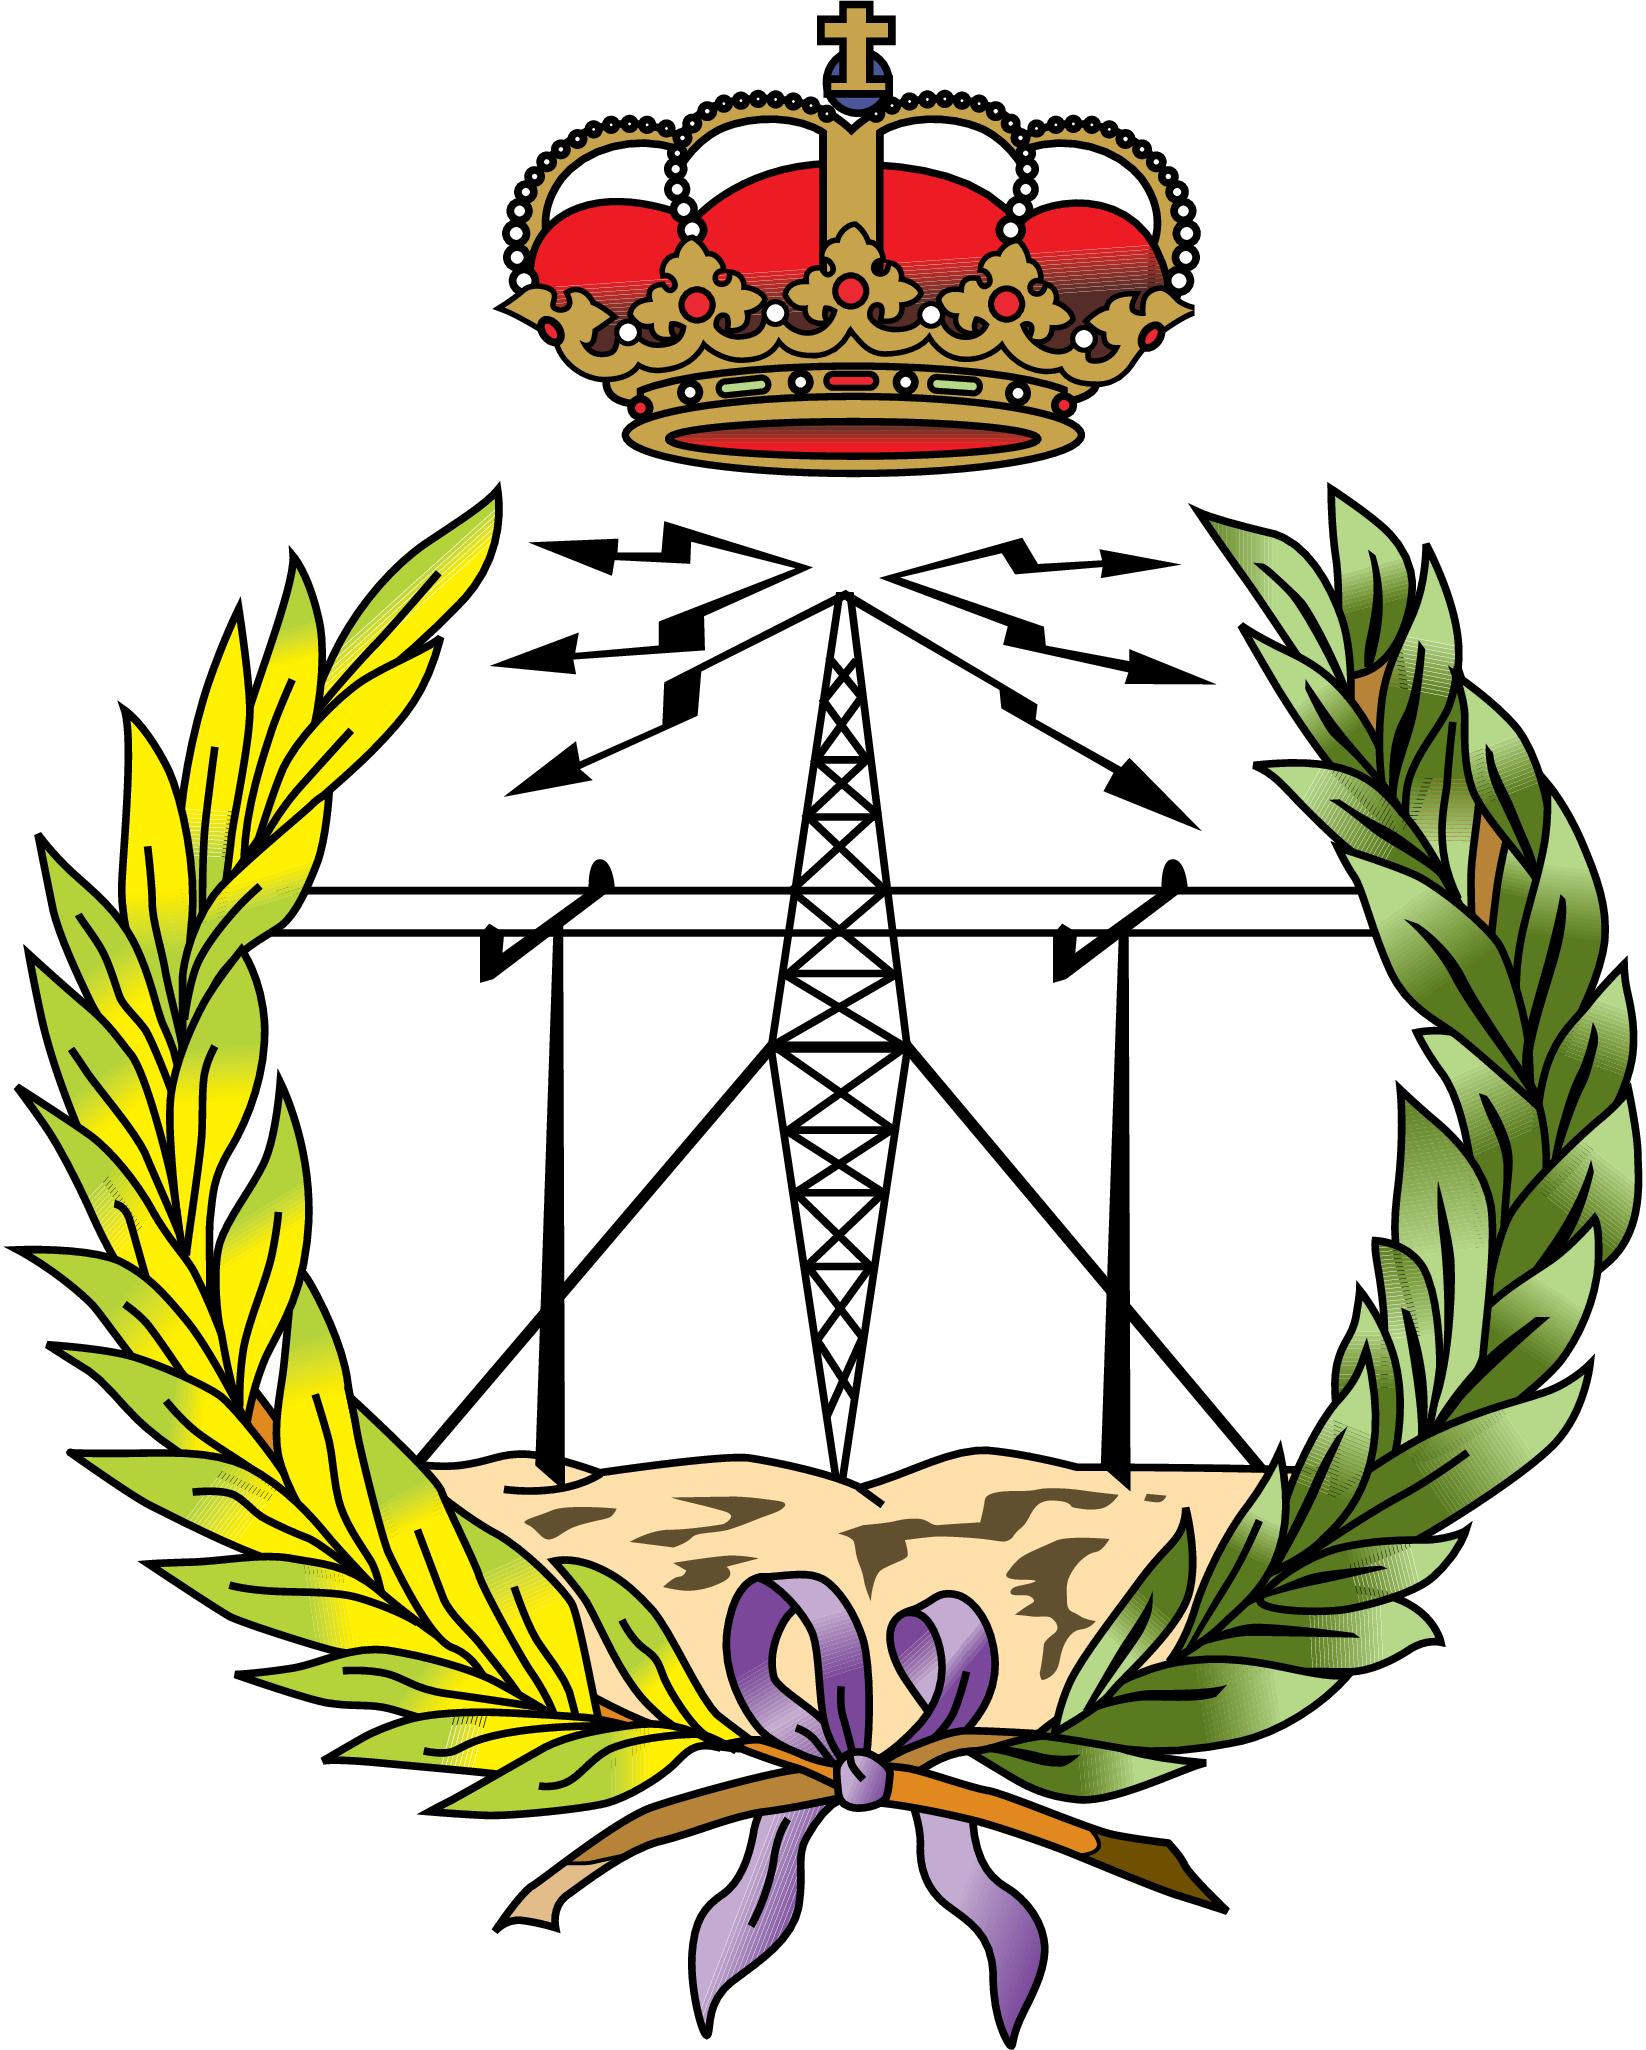
\includegraphics[width=\linewidth]{../../Archivos comunes/etsist_logo.png}
	\end{subfigure}
\end{figure}

% Introducción
\newpage
\phantomsection
\addcontentsline{toc}{section}{Introducción}
\section*{Introducción}
Imagen de la portada: \textsl{Le magie noire}, por René Magritte.

Esta asignatura es básica para cualquier ingeniería de Telecomunicaciones. Se basa principalmente en las matemáticas explicadas en Señales y Sistemas. Por ello, para las prácticas de laboratorio usaremos MATLAB.

El Bloque 1 representa el 40\%

La evaluación del laboratorio se realizará a partir de los informes de las prácticas $(50\% )$ y del examen $(50\% )$.

Teoría 90\% + LAB 10\%

Repasar presentación en powerpoint para completar introducción.

\newpage

% Índice (TOC)
\setlength{\parskip}{0em}
\tableofcontents 
\setlength{\parskip}{0.5em}

%%% INICIO DE LOS APUNTES %%%
\chapter{Modelo de sistema de comunicación}

\section{Definiciones básicas}

La \textbf{ITU} (Unión Internacional de Telecomunicaciones) nos indica la terminología que debemos usar en el ámbito de las telecomunicaciones.

\begin{description}
	 \item[Canal de transmisión:] Conjunto de medios necesarios para asegurar la transmisión de señales en un sentido entre dos puntos.
	 \item[Señal:] Fenómeno físico en el cual pueden variar una o más características para \textbf{representar información}.
	 \begin{itemize}
		  \item \textbf{Canal de frecuencia:} Parte del espectro de frecuencias que se destina a ser utilizado para la transmisión de señales y que puede determinarse por su frecuencia central y el ancho de banda asociado. 
	 \end{itemize} 
	 \item[Telecomunicación:] Tota transmisión, emisión o recepción de señales que representan signos, escritura, imágenes y sonidos o \textbf{información de cualquier naturaleza} por hilo, ondas electromagnéticas, medios ópticos u otros sistemas electromagnéticos.
	 \item[Teoría de la comunicación:] Tiene por objeto encontrar las técnicas más adecuadas que, con los condicionantes económicos, tecnológicos... permiten optimizar el \textbf{consumo de ancho de banda} (BW) y \textbf{potencia} ($P$) para poder transmitir una determinada información con una \textbf{calidad determinada}.
\end{description}

\section{Esquema funcional de un sistema de comunicación}
FALTA AÑADIR IMAGEN 

\subsection{Fuentes de información}

Las diferentes fuentes de información pueden clasificarse como:
\begin{description}
	 \item[Analógica] La información a transmitir es una señal continua en el tiempo. Cabe mencionar que las señales analógicas pueden digitalizarse. Por ejemplo, una forma de conseguirlo sería mediante cuantificación y codificación PCM (explicado más adelante, falta añadir una referencia cuando lleguemos a esa parte del temario, en el Tema 6).
	 \item[Digital] La información consiste en símbolos pertenecientes a un alfabeto finito, que se envían secuencialmente en intervalos discretos de tiempo. Los \textbf{símbolos} son los posibles valores que puede tomar. Por ejemplo, una señal digital binaria tiene dos símbolos.
\end{description}

\subsection{Transmisor}

El transmisor convierte la señal de información (fuente) en señales eléctricas o electromagnéticas (formas de onda) adecuadas para su transmisión a través del medio físico (canal de comunicaciones).

Existen varios tipos de transmisiones:

\begin{itemize}
	 \item Transmisión \textbf{banda base} $\longleftrightarrow$ Transmisión paso banda (\textbf{modulación}).
	 \begin{itemize}
		  \item En banda base: Se emite la información en la misma banda que ocupa, como se generó la fuente.
		  \item Con modulación: La banda ocupada por la información se traslada a otra más alta. Esto se hace para:
		  \begin{itemize}
			   \item Adaptar la banda transmitida a los requerimientos del canal.
			   \item Multiplexar señales. Es decir, permitir que varias compartan el mismo canal de comunicaciones. \textbf{FDM} (Multiplex por división en frecuencia).
		  \end{itemize}
	 \end{itemize}
	 \item Transmisión \textbf{analógica} $\longleftrightarrow$ Transmisión \textbf{digital}
\end{itemize}

\subsubsection{Modulación}

La señal moduladora modula una señal portadora (sinusoidal en nuestro caso)
\[ S\subtext{moduladora}(t) \]
\[ x_p(t) = A \sen \left( \omega t + \phi \right) \]
\[ \omega _c = 2\pi f_c \]

[Representación del espectro del seno]

\begingroup
\renewcommand{\arraystretch}{1.2}
\begin{center}
	\begin{tabular}{c | c | c}
		Portadora & Analógica & Digital\\ \hline
		& AM \footnotemark & ASK\\ 
		Senoidal & FM & FSK \\ 
		 & PM & PSK \\ \hline
		 & PAM o PCM & \\ 
		Cuadrada & PPM &  \\ 
		 & PWM &  \\ \hline
	\end{tabular}
\end{center}
\footnotetext{Modulación en amplitud}
\endgroup

\chapter{Caracterización de señales}

\section{Representaciones logarítmicas}

\subsubsection{Ejercicio 1}

Tenemos un canal de transmisión con un amplificador que ofrece una ganancia $G$ de $32\dB$ y un cable muy largo que afecta aplicando una atenuación $A$ de $20\dB$ a la señal. A la entrada del amplificador (punto 1), introducimos un tono con amplitud de pico $2\V$.

Rellena la tabla con los valores que se piden para cada parte del canal de transmisión.

\begin{center}
	\begin{circuitikz}
		 \draw (0,0) node[label={above:$\circledNumber{1}$}] {}
		 to[amp,l_=${G=32\dB}$,o-o] ++(3,0) node[label={above:$\circledNumber{2}$}] {} to[TL,l_=${A=20\dB}$, -o] ++(5,0) node[label={above:$\circledNumber{3}$}] {};
	\end{circuitikz}
\end{center}

\begin{center}
	\underline{\textbf{Solución}}
\end{center}

Las respuestas han sido coloreadas de color verde en la tabla, y a continuación puedes observar la resolución del ejercicio. Existen numerosas formas de llegar al resultado. Esta solución es la que se me ocurrió según lo resolvía.

\begingroup
\renewcommand{\arraystretch}{1.5}
\begin{center}
	\begin{tabular}{|c|c|c|c|}
		\hline
		 \textbf{Magnitud} & $\circledNumber{1}$ & $\circledNumber{2}$ & $\circledNumber{3}$ \\ \hline 
		 $x_p \ [\V ]$ & $2\V$ & \textcolor{green!65!black}{$79.62\V$} & \textcolor{green!65!black}{$7.96\V$} \\ \hline
		 $p \ [\W ]$ & \textcolor{green!65!black}{$0.04\W$} & \textcolor{green!65!black}{$63.4\W$} & \textcolor{green!65!black}{$0.0634\W$} \\ \hline
		 $P \ [\dBW ]$ & \textcolor{green!65!black}{$-10.97\dBW$} & \textcolor{green!65!black}{$18\dBW$} & \textcolor{green!65!black}{$-2\dBW$} \\ \hline
		 $P \ [\dBm ]$ & \textcolor{green!65!black}{$19.03\dBm$} & \textcolor{green!65!black}{$48\dBm$} & \textcolor{green!65!black}{$18\dBm$} \\ \hline
	\end{tabular}
\end{center}
\endgroup

Podemos calcular $p_1$ sabiendo que la potencia de un tono es la siguiente:
\[ p_1 = \frac{x_p^2}{2R} = \frac{2^2}{2 \cdot 50} = 0.04\W \]

Por lo tanto:
\begin{align*}
	P_1 [\dBW] &= 10 \log \left( 0.04 \right) = -14\dBW \\ 
	P_1 [\dBm] &= 10 \log \left( 40 \right) = 16\dBm
\end{align*}

De aquí, podemos obtener el resto de potencias logarítmicas:
\begin{align*}
	P_2 [\dBW] &= P_1[\dBW] + G = -14 + 32 = 18\dBW \\ 
	P_2 [\dBm] &= P_1[\dBm] + G = 16 + 32 = 48\dBm\\[5pt]
	P_3 [\dBW] &= P_1[\dBW] + A  = -14\dBW \\ 
	P_3 [\dBm] &= P_1[\dBm] + A  = 16\dBm
\end{align*}


\section{Caracterización Temporal}
\section{Caracterización Espectral}

\subsection{Densidad esoectral de potencia}

La densidad espectral de potencia $G_x(f)$ mide la potencia de la señal por unidad de ancho de banda $\left( \W / \Hz \right)$.

En un sistema LTI con respuesta en frecuencia $H(f)$, la densidad espectral a la salida se puede calcular como:
\[ \boxed{G_y(f) = G_x(f) \cdot \abs{H(f)}^2} \]

\subsubsection{Ancho de banda}

El \textbf{ancho de banda a 3 dB} se mide entre las frecuencias donde la potencia es la mitad con respecto al máximo.

el \textbf{ancho de banda equivalente} es el ancho de un espectro rectangular ficticio que contendría la misma potencia que la señal original. Es decir, que tiene potencia equivalente. [añadir imagen]

El \textbf{ancho de banda entre nulos} se explicará con más detalle en el Tema 7 [falta referencia]

\section{Señales habituales}

\subsection{Señal triangular}

\subsection{Señal cuadrada}

\chapter{Ruido térmico}
\section{Caracterización del ruido térmico}
\section{Caracterización del ruido en cuadripolos y dipolos}
\section{Fórmula de Fris}
\section{Modelo de un Analizador de Espectros}

\chapter{Distorsión}
\section{Tipos de distorsión}
\section{Distorsión lineal}
\section{Distorsión no lineal}

\chapter{Modulaciones analógicas}
\section{Concepto de modulación y tipos}
\section{Modulaciones lineales: AM, DBL}
\section{Modulaciones angulares: FM}
\section{Calidad}

\chapter{Conversión A/D y codificación PCM}
\section{\texorpdfstring{Elementos de un sistema de comunicaciones\\ digitales}{Elementos de un sistema de comunicaciones digitales}}
\section{Conversión A/D}
\section{Cuatificación uniforme y no uniforme}
\section{Multiplez por División en el Tiempo (TDM)}

\chapter{Transmisión digital por canales de ancho de banda limitado}
\section{Modelo de Transmisión Digital}
\section{Ancho de banda de señales banda base}
\section{Interferencia entre símbolos (ISI)}
\section{Criterio de Nyquist}
\section{Filtrado en coseno alzado}
\section{Diagrama de ojos}
\section{Códigos de línea}

\chapter{Transmisión digital banda base con ruido}
\section{Representación geométrica de señales}
\section{\texorpdfstring{Implementaciones del receptor: correlador, filtro\\ atrapado}{Implementaciones del receptor: correlador, filtro atrapado}}
\section{Teoría de la Detección (receptor binario óptimo)}
\section{Probabilidad de error en sistemas binarios}
\section[\texorpdfstring{Ejemplos de expresiones de probabilidad de error para varias\\ señalizaciones binarias}{Ejemplos de expresiones de probabilidad de error para varias señalizaciones binarias}]{Ejemplos de expresiones de probabilidad de error para varias señalizaciones binarias}

\addtocontents{toc}{\vfill}
\addtocontents{toc}{\protect\pagebreak}
\chapter{Modulaciones digitales}
\section{Modulaciones lineales. Fórmulas básicas}
\section{ASK}
\section{PSK}
\section{QAM y APK}
\section{FSK}
\section{Comparación entre modulaciones digitales}
%%% FIN DE LOS APUNTES %%%

%%% BIBLIOGRAFÍA %%%
% Por defecto, se encuentra desactivada. Esto disminuye el tiempo de procesado. Se puede activar cuando se vaya a exportar el PDF definitivo

%\newpage
%\phantomsection
%\label{sec:bibliografia_final}
%\renewcommand{\refname}{Bibliografía}
%\addcontentsline{toc}{section}{Bibliografía}
%\bibliography{bibliografia} % Nombre del archivo (sin ".bib")
%\bibliographystyle{bababbrv}

\end{document}
